

\newsavebox{\boxReviList}
\begin{lrbox}{\boxReviList}
\begin{minipage}[c]{0.4\linewidth}
\begin{alltt}
([0 Revi_00, Revi_01, ...]
 [1 Revi_10, Revi_11, ...]
 ...
 [n Revi_n0, revi_n1, ...])
\end{alltt}
\end{minipage}
\end{lrbox}

\newsavebox{\boxSendiList}
\begin{lrbox}{\boxSendiList}
\begin{minipage}[c]{0.4\linewidth}
\begin{alltt}
((0 [1 Sendi_100, Sendi_101, ...], [2 Sendi_200, Sendi_201, ...], ...)
 (1 [0 Sendi_010, Sendi_011, ...], [2 Sendi_210, Sendi_211, ...], ...)
 ...
 (n [0 Sendi_0n0, Sendi_0n1, ...], [1 Sendi_1n0, Sendi_1n1, ...], ...))

\end{alltt}
\end{minipage}
\end{lrbox}

\section{ Over-approximated Match-pair Generation}

%In order to apply the $\mathbf{ans}$ function to correctly analyze the behaviors of a CTP, the CTP and a set of match pairs must be provided as inputs. In this section, we present two sets of match pairs. The first set is a precise set of match pairs, the one that contains no match pairs that cannot legally occur in an execution of the CTP and contains each match pair that could possibly occur in any execution of the CTP. We call this set $mp_{\phi}$. The $\mathbf{ans}$ function can use $mp_{\phi}$ to correctly analyze the CTP without underapproximating or overapproximating its behaviors. On the other hand, the other set, $mp$, contains all the match pairs that can possibly occur in any execution of the CTP, together with some match pairs that can not legally occur in the execution of the CTP. As a result, $mp$ can overapproximate the behaviors of the CTP. The overapproximation does not stop us from correctly analyzing the behaviors of the CTP because we can increasingly modify the contents of the set in a loop of refinement with low cost (Or we could say that The SMT solver will handle the bogus match pairs??). We will present the process of abstract refinement loop in the later section(??). In this section, we will also present two methods that generate both sets. Both algorithms are not computability efficient since the fastest one requires at least quadratic computational complexity, but we present them to make a complete treatment of the subject. In the later section we will discuss how this computationally expensive process might be avoided.

In the previous sections, we know that a precise set of match pair and a CTP is required to verify all possible execution traces through a SMT problem. Generating a precise set of match pair is time consuming because an execution tree needs to be generated, which requires exponential time complexity to finish. It is impossible to verify a regular MCAPI program because of the state explosion. In this section, we present a method that over-approximates the set of match pair, such that match pairs that can exist in the real execution are all included, and some bogus match pairs that can not exist in the execution are also included and required to prune. We then input this over-approximated set of match pair to a CEGAR loop for further verification. Either error is found during one iteration and the process stops, or the current set of match pair is prune to a more precise one for the next iteration. 

%\subsection{Precise Match-pair Generation}

%The generation of $mp_{\phi}$ is completed by performing a modified depth-first search traversal over the CTP. For convenience, we assume that the provided CTP consists of the Rcvi and Sndi commands with the same size. $N$ represents the size of Rcvi commands and Sndi commands in the CTP. Also, for each Rcvi command in the set of Rcvi, no matter what execution sequence there occurs, there exists at least one Sndi command that matches the Rcvi command, and vice versa. $S$ represents each node(State) in the depth-first search tree, and maintains a copy of two lists, where the first one stores the pending Rcvi commands and the second one stores all the pending Sndi commands. we illustrate the structure of both lists in \figref{fig:data-structure-pendinglist}.

 %In \figref{fig:data-structure-pendinglist}, the Rcvi list is defined as a Hash set where each entry is a sublist of pending Rcvi commands and the key of the entry represents the corresponding thread ID (end-point) of those Rcvi commands.
%The Sndi list is defined as a nested Hash set, where each entry contains a few sublists of Sndi commands with the same destination thread (to-end-point). The key of the entry represents the to-end-point of all Sndi commands in the entry. Also, each sublist of Sndi commands has the same source thread (from-end-point). Thus, the Sndi commands from the same sublist are from the same thread, and are able to send to the same thread. $S$ can be updated by inputting new pending Sndi or Rcvi commands from the original CTP and completing matching some Sndi with some Rcvi commands (by deleting from the pending lists). The algorithm works as follows:

\begin{figure}
%\begin{center}
\setlength{\tabcolsep}{7pt}
%\begin{tabular}{l}
\scalebox{0.68}{\usebox{\boxReviList}} \\
\begin{center}
(a)
\end{center}


\scalebox{0.68}{\usebox{\boxSendiList}} \\
\begin{center}
(b)
\end{center}
%\end{tabular}
%\end{center}
\caption{Structure of pending lists. (a) List of Rcvi commands. (b) List of Sndi commands.}
\label{fig:data-structure-pendinglist}
\end{figure}

%\begin{itemize}
%\item[1] Build the initial state, which is also denoted as the root of the search tree, by traversing across each thread in the original CTP. When a Rcvi command is encountered the command is added to a set of pending Rcvi commands, and the scanning of that thread pauses. If a Sndi command is encountered the command is added to a set of pending Sndi commands, and the scanning of that thread continues. Any other commands are simply ignored.
%\item[2] The pending Revi and Sndi commands are then checked whether the end-point of the Revi command is equivalent to the to-end-point of the Sndi command. If a possible match pair exists, a new state(node of the search tree) is generated by deleting the Revi and Sndi commands of the match pair from the pending lists and continuing scanning the paused treads in the CTP using the same rules above.
%\item[3] Repeating step 2 until we generate a leaf node, where the pending list is empty and all the threads are scanned. When a leaf node is generated, one possible execution sequence is simulated for the original CTP. The search will backtrack to some internal state so that other branches can be scanned.
%\item[4] Repeating step 2 and 3 until we can finish the depth-first search traversal and storing all possible match pairs.
%\end{itemize}

%The generated set of match pairs are guaranteed to be the precise set we mentioned in the previous paragraph because of the fact that it is generated from the simulation of the real execution of the CTP. \figref{fig:search_tree} illustrates the generated depth first search tree of the example CTP in \figref{fig:mcapi}, where each node represents the state generated, and the label on each edge represents a match pair found when generating the nodes.
%\begin{figure}
%Need figure here
\begin{comment}
   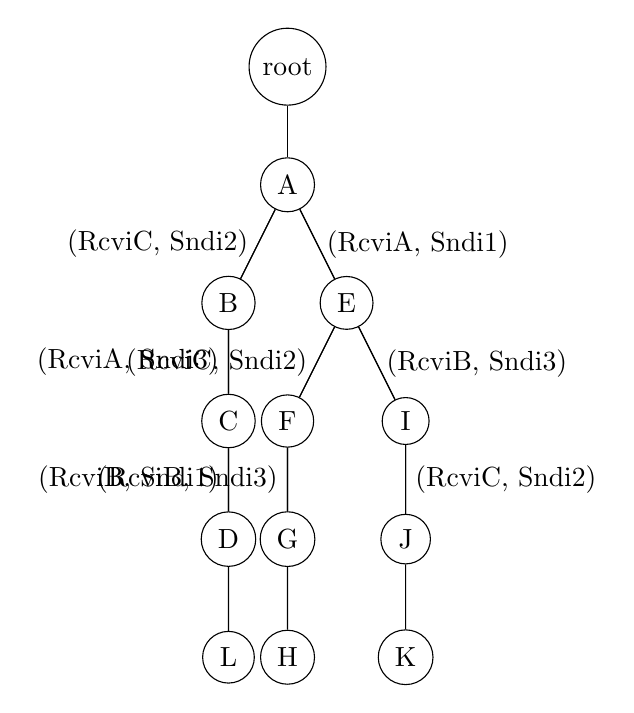
\begin{tikzpicture}
   \tikzstyle{every node}=[circle,draw]
\node(root) {root}
  child{ node(A) {A}
        child{node(B) {B} child{node(C) {C} child{node(D){D} child{node(L){L}}}}}
        child{node (E) {E}
                child{node(F){F} child{node(G){G} child{node(H){H}}}}
                child{node(I){I} child{node(J){J} child{node(K){K}}}}}};

\tikzstyle{every node}=[->]
\path
(root) edge node[right]{} (A)
(A) edge node[left]{(RcviC, Sndi2)} (B)
    edge node[right]{(RcviA, Sndi1)} (E)
(B) edge node[left]{(RcviA, Sndi3)} (C)
(C) edge node[left]{(RcviB, Sndi1)} (D)
(E) edge node[left]{(RcviC, Sndi2)} (F)
    edge node[right]{(RcviB, Sndi3)} (I)
(F) edge node[left]{(RcviB, Sndi3)} (G)
(I) edge node[right]{(RcviC, Sndi2)} (J);

\end{tikzpicture}
\end{comment}
%\caption{An example of Depth-first Search Tree for the CTP}
%\label{fig:search_tree}
%\end{figure}


%\subsection{Overapproximated Match-pair Generation}

Other than simulating all possible executions of the CTP, the algorithm that generates the over-approximated match pairs is basically a strategy of matching and pruning among all possible Sndi and Rcvi commands with matched end points. We use the structure in \figref{fig:data-structure-pendinglist} to support the algorithm. We keep one copy of both lists and store the Rcvi and Sndi commands as follows: The Rcvi commands in all threads are scanned and stored in the list of Rcvi, where the index of a Rcvi command, $r_i$, is the actual order in the thread where this Rcvi command exists. For example, $Rcvi(t_0, i)$ represents the $i_{th}$ Rcvi command in Thread $t_0$. Similarly, the Sndi commands in all threads are stored and ordered in the list of Sndi, where $s_i$ is the index of a Sndi command in the sublist of Sndi commands with same from-end-point and to-end-point. For example, $Sndi(t_0, t_1, j)$ represents the $j_{th}$ Sndi command sending from $t_1$ to $t_0$. In addition, we have the following lemma that supports the pruning strategy in the algorithm.



\begin{lemma}
For each Rcvi command with index $r_i$ and all matched Sndi commands of this Rcvi command, if $s_j$ is the index of any Sndi commands,
\begin{itemize}
\item[1.] $r_i \geq s_j$;
\item[2.] $r_i \leq s_j + (N - sendsize_j)$.
\end{itemize}
Where $N$ is the number of Sndi commands in all threads, and $sendsize_j$ is the size of the sublist where this Sndi command exists.
\label{lemma:Rcvi_Sndi_index}
\end{lemma}
%\begin{proof}
%We prove it by contradiction. Suppose statement $1$ is not satisfied for some match pair $(Rcvi, Sndi)$, so $r_i < s_j$. Since the Sendi commands with the same from-end-point and to-end-point are sent in a FIFO way, where the first Sndi command should be served first in the destination thread. It is impossible for any strategy to match all those Sendi commands with index less than $s_j$ with some commands because there exist at least one extra Sndi command that can not match any Rcvi command with index less than $r_i$. The contradiction occurs. Thus, statement $1$ is proved.

%Similarly, Statement $2$ is not satisfied implies that $r_i > s_j + (N - sendsize_j)$ for the match pair $(Rcvi, Sndi)$. $(N - sendsize_j)$ represents the size of all Sndi commands with from-end-point $j$ and to-end-point other than i. Because of the same reason in the last paragraph, we can not find a strategy that match all Sndi commands with index large than $s_j$ sending from thread $j$ to thread $i$. Thus, the contradiction occurs and statement $2$ is proved.

%\end{proof}

The algorithm that generates the over-approximated set of match pairs works as follows:
\begin{itemize}
\item[1] For each Rcvi command $Rcvi(t_s, i)$, all Sndi commands in the entire set of sublists $SndiList(t_s)$ are selected as candidates for matching the Rcvi command.
\item[2] For each candidate Sndi command $Sndi(t_s, t_d, j)$, check if \lemmaref{lemma:Rcvi_Sndi_index} is satisfied. If it is satisfied, the pair $(Rcvi(t_s, i), Sndi(t_s, t_d, j))$ is added to the result set of match pairs. Otherwise, this pair is ignored, and other candidate Sndi commands for $Rcvi(t_s, i)$ are checked.
\item[3] Repeat step 1 and 2 until each Rcvi command is checked with all its candidate Sndi commands.
\end{itemize}

The generated set of match pairs is an over-approximation of the precise set because it contains all legal match pairs. Furthermore, the pruning strategy restricts the size of the set because some match pairs that can illegally exist are removed.

Now, we analyze the time complexity of this algorithm, which requires several steps to complete. Organizing the contents of pending lists requires linearly scanning the CTP so that the time complexity for this step is $O(N)$. Matching the possible Sndi commands with the given Rcvi commands requires $N_0^2 + N_1^2 + ... + N_n^2 < N^2$ steps, where $N_0 + N_1 + ... + N_n = N$, so this step requires $O(N^2)$ time complexity. Thus, the whole process requires $O(N^2)$ time complexity totally. %The modified depth first search approach relies on the process of generating and updating the nodes(states) of the search tree, thus, the time complexity is $O(b^N)$, where $b$ is the branching factor. The variation of the branching factor $b$ depends largely on the structure of the CTP. For example, the search tree in \figref{fig:search_tree} can be compressed if the program orders of commands in the scenario are changed.

%\subsection{Stuff needs to be modified}
%\begin{itemize}
%\item In fist paragraph, how do we claim that an over-approximated set of match pairs is useful?
%\item The figure of the example search tree needs to be modified.
%\item Do we need to explain the example tree?
%\item The figure of the structure of pending lists should be modified. How to write the math expression in the box?
%\item Is the analysis of the time complexity correct?
%\end{itemize}
